\Chapter{EXTRACTION DE TAXONOMIE EXPRESSIVE}
\label{chap:texp}

\section{Motivation et principes généraux}

Dans la section précédente, on a décrit une méthode pour extraire une hiérarchie entre les types à partir des seuls plongements d'entité. 

Méthode précédente : on s'interdit d'utiliser le linked data => comment retrouver l'information connue (la taxonomie DBpédia) à partir des seuls plongements vectoriels ?

Cette méthode : en utilisant toute l'information accessible, comment aller plus loin que ce qui existe (en l'occurence, trouver une taxonomie expressive – qui à l'heure actuelle n'existe pas)

Pas d'utilisation du Linked Data = méthode très descriptive, qui n'utilise pas toute l'information à notre disposition.

Schéma général proche de la méthode précédente : regroupement hiérarchique sur les entités, puis transformation de la hiérarchie entre entités en une hiérarchie sur les classes. Ici, étiquettage de la classe plus sophistiqué, puisuq'on s'autorise Linked Data

Pourquoi ça marche ? Parce qu'on travaille sur un groupe d'entités dont on sait qu'elles sont sémantiquement proches, de par la géométrie de leurs plongements. Donc on restreint la dimension de l'espace de recherche, qui est un goulot d'étranglement habituel des méthodes d'extraction d'axiomes.

Toutefois, un ajout majeur : le retirage récursif des entités à regrouper pour limiter la propagation des erreurs dans l'arbre, limiter le bruit et affiner progressivement la spécificité des classes extraites. Plus un \textit{bag of tricks} pour que ça marche bien.

\paragraph{Remarque}

DBpédia, comme la plupart des graphes de connaissances, fonctionne sous l'hypothèse du monde ouvert : si un triplet est absent du graphe, cela ne signifie pas nécessairement qu'il est faux. Aussi, dans la suite, lorsqu'on écrit qu'une entité $x$ ne vérifie pas un prédicat logique $P$, cela doit être compris comme un raccourci pour écrire que l'assertion $P(x)$ n'est pas contenue dans le graphe, et non comme l'assertion $\neg P(x)$.

\section{Méthode proposée}
\subsection{Regroupement hiérarchique récursif avec retirage}

La méthode d'extraction de taxonomie expressive commence elle aussi par une phase de regroupement hiérarchique. Dans la méthode précédente, on avait comme seules données d'entrée un ensemble fixé d'entités typées $\cal{D}$. Ici au contraire, on s'autorise l'accès à tout le graphe, donc l'ensemble $\cal{D}$ sur lequel s'opère le regroupement hiérarchique est variable et change au cours de l'exécution de l'algorithme. À chaque étape $t$, on effectue un regroupement hiérarchique sur les plongements des entités de $\cal{D}_t$, puis on étiquette les clusters obtenus avec des axiomes logiques (l'extraction d'axiomes à partir de clusters est détaillée dans la section \ref{subsec:texp-exaxiom}). Chaque nouvel axiome extrait sert alors à créer un nouveau jeu de données, sur lequel on répète l'étape précédente, ce qui permet d'étendre itérativement la taxonomie prédite.

% Ensuite, pour chacun des axiomes $a_1, \ldots, a_k$ obtenus, on tire aléatoirement des entités qui vérifient cet axiome, ce qui donne de nouveaux ensembles d'entrées $\cal{D}_{t+1}, \ldots, \cal{D}_{t+k}$.

Dans cette section, on se donne une fonction d'extraction d'axiome $\alpha$, telle que $\alpha(C)$ est un axiome logique qui qualifie le cluster $C$, si un tel axiome existe, et qui renvoie un symbole spéciale \texttt{indéfini} dans le cas contraire. Un exemple d'une telle fonction est donné dans la section suivante. 

% Principe général
On dispose d'une file d'axiomes à traiter $A$, et de la taxonomie en cours de construction $\Tpred$. La file d'axiomes à traiter n'est autre que la liste des feuilles de $\Tpred$ qui n'ont pas encore été visitées. Lorsqu'on visite un axiome $\alpha$ de $A$, soit on parvient à extraire un sous-arbre $T_\alpha$ qui contient des axiomes, et alors $T_\alpha$ est ajouté à $\Tpred$ à l'emplacement de $\alpha$, et les nœuds feuilles de $T_\alpha$ sont ajoutés à la file des axiomes à traiter; soit on ne trouve aucun sous-axiome pertinent pour $\alpha$, auquel cas $\alpha$ reste une feuille de $\Tpred$ et la recherche continue dans les autres axiomes de la file $A$, jusqu'à épuisement de $A$.

Pour la première étape, $A$ est initialisée à $\{\top\}$ : le seul axiome de $A$ est le concept universel $\top$ qui, par définition, est vérifié par toutes les entités du graphe. $\top$ sert de racine à la taxonomie, puisque c'est le seul axiome dont on soit sûr \textit{a priori} qu'il définisse toutes les entités.
La taxonomie $\Tpred$ est réduite à un seul sommet $\top$ et ne contient donc aucune arête. 

Tant que la file $A$ n'est pas vide, on retire son premier élément $a$, qui sert d'axiome d'entrée pour cette étape. On prélève aléatoirement, dans le graphe $\KG$, $N$ entités parmi celles qui vérifient $a$ – dans notre implémentation, le graphe est représenté \textit{via} une librairie Python spécifique, mais dans d'autres contextes, le langage de requête SPARQL pourrait être utilisé à cette fin. Les plongements de ces entités donne un nuage de points $\cal{D}_a$ de dimension $d \times N$, avec $d$ la dimension des entités.

Sur ce nuage de point $\cal{D}_a$, on effectue un regroupement hiérarchique, comme décrit dans la section \ref{subsec:te-clustering}. À nouveau, on considère deux choix de paramètres de cet algorithmes : distance euclidienne avec critère de Ward, et distance cosinus avec liaison moyenne. La première fusionne les clusters de façon à minimiser la variance du nouveau cluster créé. À l'étape $t$, notons $\cal{C}_t$ les clusters existant; les clusters $C_1$ et $C_2$ à fusionner sont choisis selon l'équation :
\begin{equation}
    C_1, C_2 = \argmin_{C_1, C_2 \in \cal{C}_t} 
    \frac{1}{| C_1 + C_2 |} \sum_{\bf{e} \in C_1 \cup C_2} \| \bf{e} - \frac{1}{| C_1 + C_2 |} \sum_{\bf{e'} \in C_1 \cup C_2} \bf{e'} \|_2^2 
\end{equation}
La seconde fusionne les clusters dont les entités ont la distance moyenne la plus faible. On fusionnera donc $C_1$ et $C_2$ tels que :
\begin{equation}
    C_1, C_2 = \argmin_{C_1, C_2 \in \cal{C}_t} \frac{1}{|C_1| \times |C_2|} \sum_{\bf{e_1}\in C_1} \sum_{\bf{e_2} \in C_2} d_\text{cos}(\bf{e_1, e_2})
\end{equation}

Le résultat est un arbre binaire, noté $X_a$, dont la racine est $\cal{D}_a$ tout entier, et dont les feuilles sont les $N$ éléments de $\cal{D}_a$. 

On effectue alors un parcours de l'arbre $X_a$, en excluant la racine $a$ qui est déjà étiquettée : pour un cluster $C$, on calcule $\alpha(C)$ pour trouver l'axiome associé à $C$. Si $\alpha(C) = \texttt{indéfini}$, le cluster $C$ n'a pas de signification logique accessible, et on poursuit la recherche dans les sous-clusters. Au contraire, si $\alpha(C)$ existe, on interrompt la recherche, et on ajoute $\alpha(C)$ à la file d'axiomes à visiter. Au-delà d'une certaine profondeur $D_\text{max}$ dans l'arbre, on arrête la recherche. On note $L_\alpha(a)$ l'ensemble des cluster $C$ étiquettés rencontrés lors de la recherche.

Finalement, on construit la sous-taxonomie extraite $T_a$ à partir de $X_a$ en suivant la procédure décrite à la section \ref{subsec:te-taxconstruction} : $T_a$ ne contient que les sommets de $X_a$ qui sont étiquettés, et qui laisse la relation de succession entre clusters inchangée :
\begin{align}
    T_a = (&\{C \in X_a : \alpha(C) \neq \texttt{indéfini}\}, \nonumber \\
    &\{(C, C' \in X_a : \exists C_1, \ldots, C_k \in X_a, \alpha(C_1) = \ldots = \alpha(C_k) = \texttt{indéfini} \nonumber \\
    &\text{ et } C \prec C_1 \prec \ldots \prec C_k \prec C'\})
\end{align}
Autre formulation\todo{choisir entre les deux notations} :
\begin{align}
    T_a = (L_\alpha(a), \nonumber 
    \{(C, C' \in X_a : \exists C_1, \ldots, C_k \in X_a \setminus L_\alpha(a), C \prec C_1 \prec \ldots \prec C_k \prec C'\})
\end{align}

Enfin, si au moins l'une des feuilles de $X_a$ n'est pas couverte par un axiome $\alpha(C)$, c'est-à-dire s'il existe au moins une branche allant des feuilles à la racine qui ne contient pas d'étiquette, c'est qu'une partie de l'arbre n'a pas été décrite par un axiome, et qu'il reste potentiellement de nouveaux axiomes à extraire. Dans ce cas, un nœud spécial \texttt{<?>} est ajouté à $T_a$ et relié directement à $a$. La signification logique de ce nœud s'écrit :
\begin{equation}
    \texttt{<?>} = a \land \left( \bigwedge\limits_{C \in L_\alpha(a)} \neg \alpha(C) \right)
    \label{eq:texp-special-node}
\end{equation}
Soit, en langage courant, l'ensemble des éléments qui vérifient $a$ mais ne vérifient aucun des sous-axiomes $\alpha(C)$ de $a$. Cette définition purement négative n'est pas d'une grande utilité dans une taxonomie expressive, puisqu'elle exprime simplement la tautologie $C \sqsubset \neg C = \top$. On utilise donc le symbole \texttt{<?>} pour signifier que la recherche n'est pas encore finie pour $a$ et qu'il reste des sous-axiomes de $a$ à trouver.

Si $T_a = (\varnothing, \varnothing)$, c'est-à-dire qu'aucun axiome n'a été trouvé en parcourant l'arbre $X_a$, alors $a$ n'aura pas de sous-axiome dans la taxonomie extraite et restera une feuille de $\Tpred$. Sinon, on remplace le nœud $a$ de $\Tpred$ par la sous-taxonomie $T_a$. On répète alors l'étape précédente, tant que la file d'axiomes $A$ n'est pas vide.

\paragraph{Le cas des nœuds spéciaux \texttt{<?>}} Dans l'étape précédente, le cas où l'axiome de départ $a$ est l'axiome spécial \texttt{<?>} est traité un peu différemment du cas général. Les données d'entrées sont toujours tirées aléatoirement, suivant la formule \ref{eq:texp-special-node}; le regroupement hiérarchique et l'extraction de la sous-taxonomie $T_a$ suit une procédure identique. Ensuite, on rattache $T_a$ à $\Tpred$. La taxonomie $\Tpred$ en cours d'extraction contient alors toujours le nœuds spécial \texttt{<?>}, qu'on ne souhaite pas garder : on modifie alors $\Tpred$ en rattachant directement les successeurs directs de \texttt{<?>} avec le prédecesseur direct de \texttt{<?>}, on ré-écrit donc les chemins $\alpha \rightarrow \texttt{<?>} \rightarrow \beta$ en $\alpha \rightarrow \beta$, et on supprime \texttt{<?>} de $\Tpred$.

\todo{Insérer une figure pour expliquer cette étape}

\begin{figure}
    \centering
    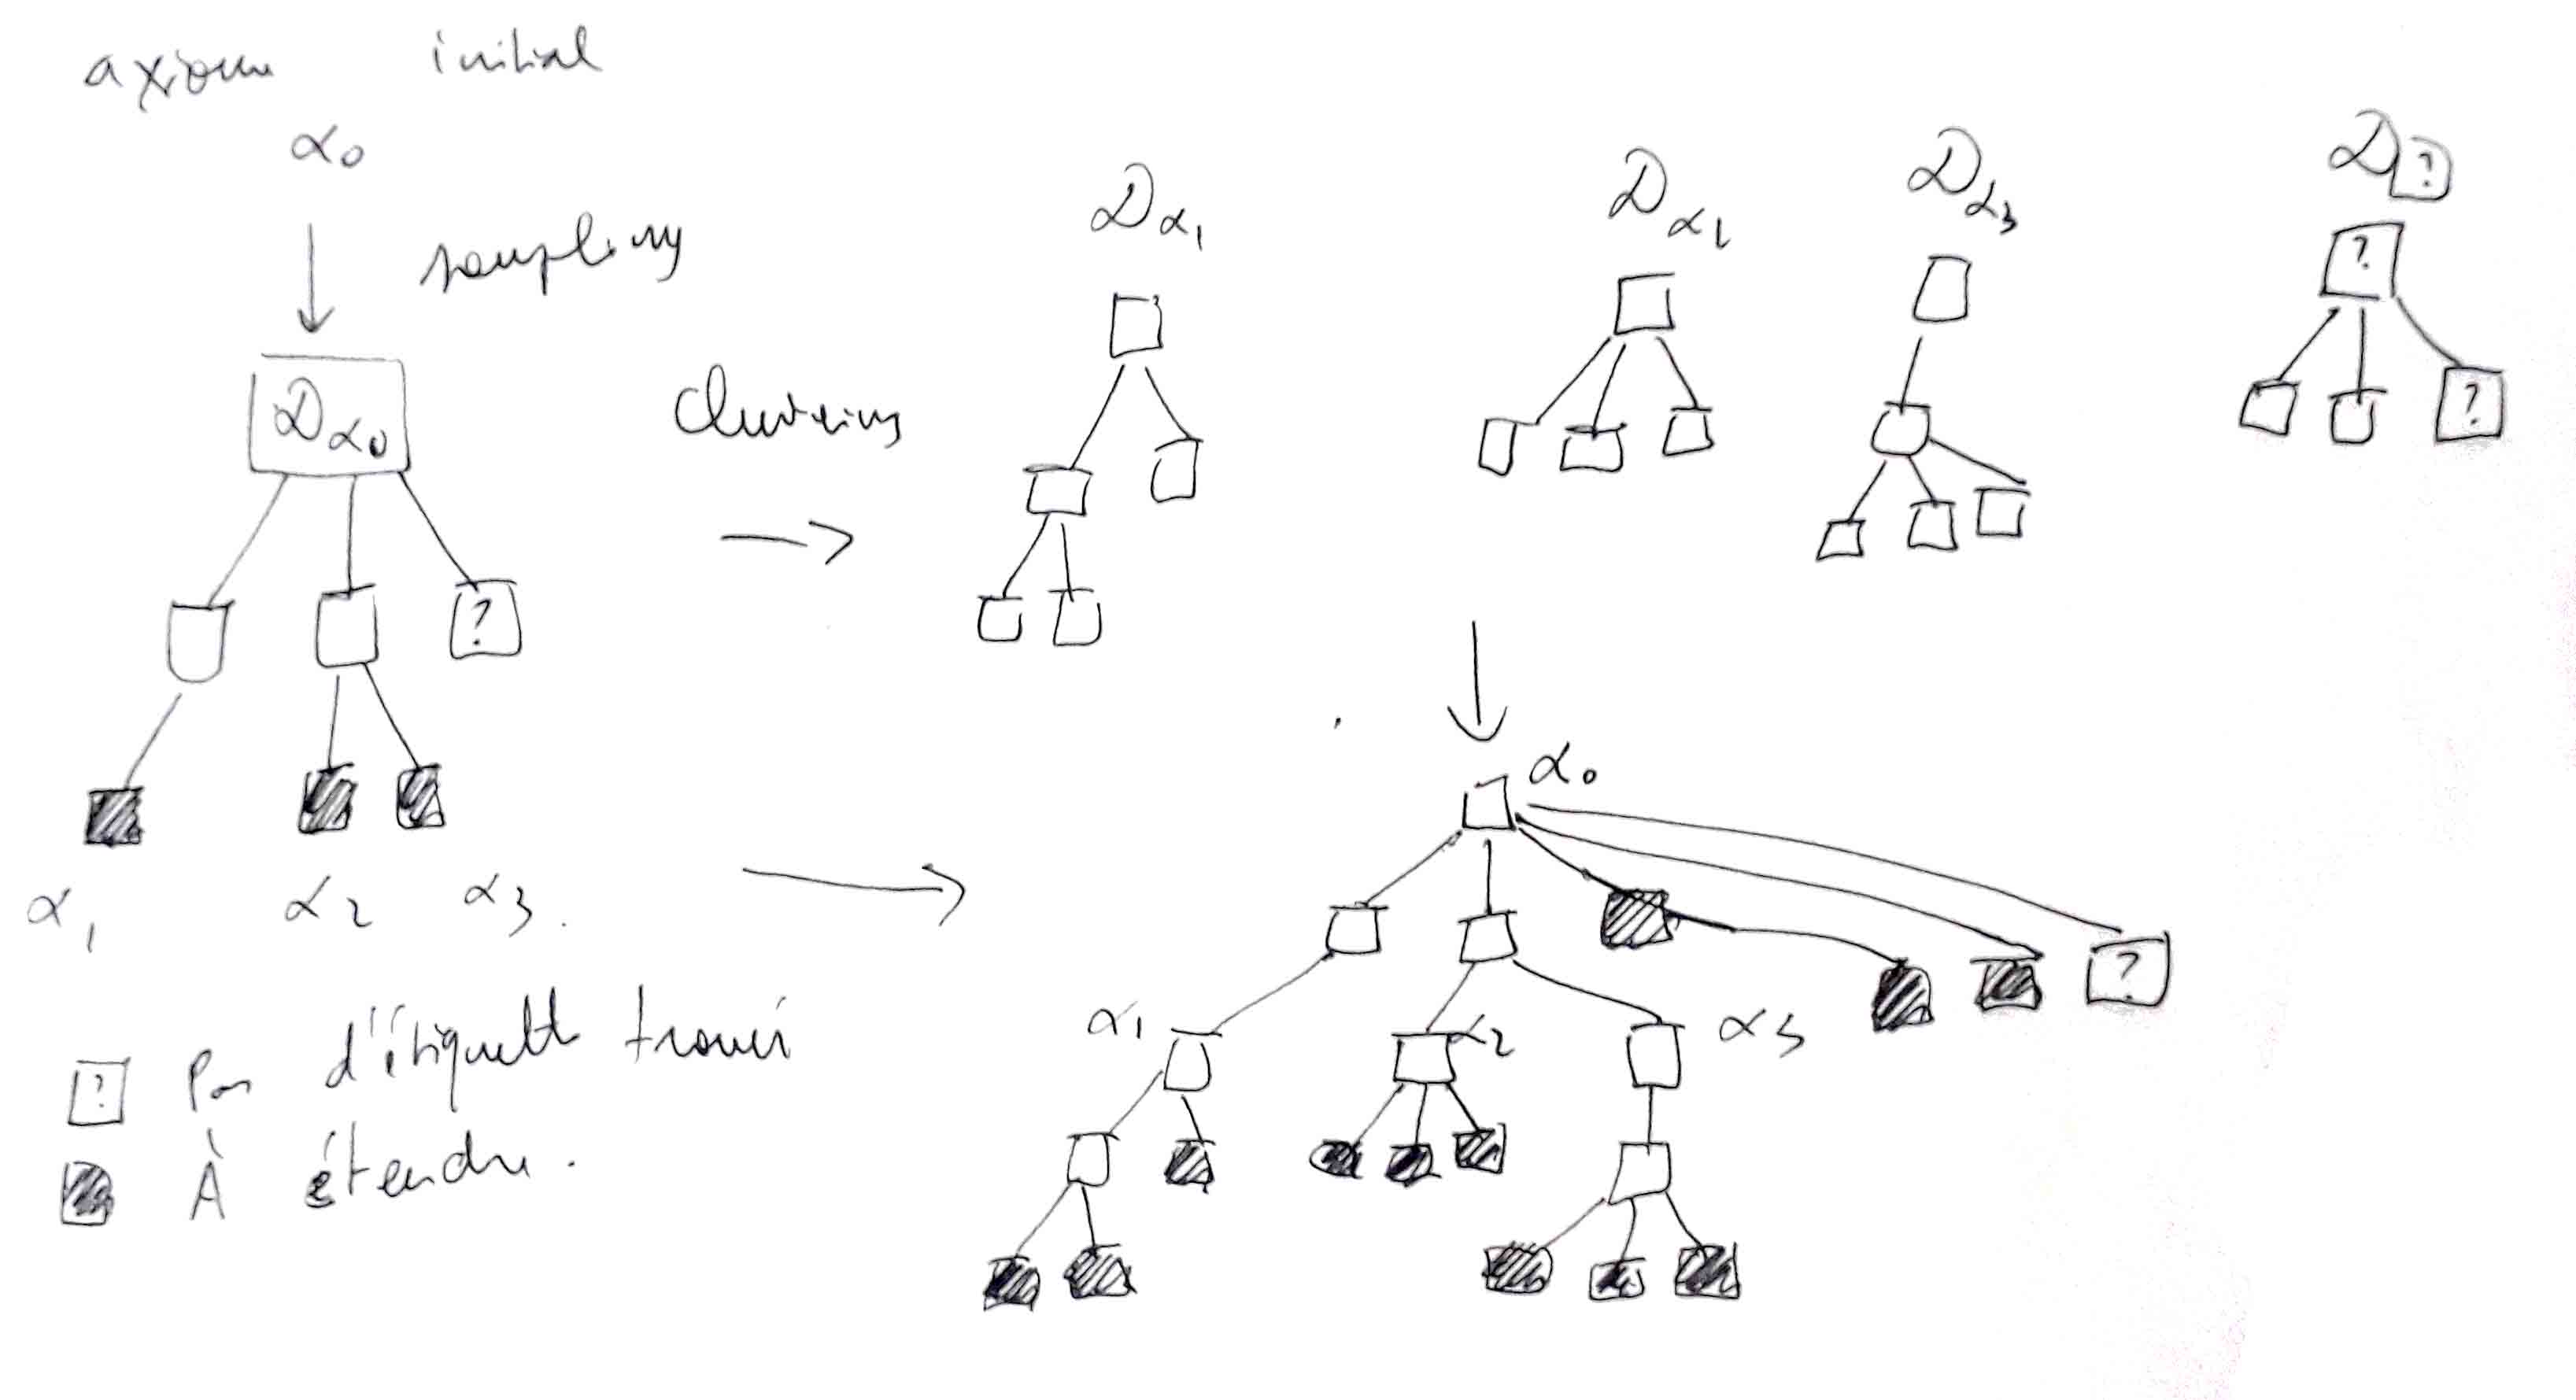
\includegraphics[width=\textwidth]{img/expressive_extraction_overview.jpg}
    \caption{(Provisoire) Principe général pour l'expansion d'arbres. À partir d'un axiome initial $\alpha_0$, un arbre est construit, et trois nouveaux axiomes $\alpha_1, \alpha_2, \alpha_3$. Trois nouveaux arbres sont construits, et ajoutés à l'arbre initial. Le procédé est répété, jusqu'à obtenir une taxonomie expressive complète.}
    \label{fig:my_label}
\end{figure}
\todo{Insérer la vraie figure pour l'expansion d'arbre}

\paragraph{Seuil adaptatif} On expérimente également une variante de l'algorithme précédent, dans laquelle le seuil $\delta$ pour l'extraction d'axiome varie au cours du temps : au début, le seuil de validité des axiomes est fixé à une valeur initiale élevée $\delta = \delta_\text{init}$; puis, à chaque fois que la file d'axiome $A$ est vidée, on diminue $\delta$ d'une quantité $d\delta$, on ré-initialise $A = \{ \top \}$, et on recommence l'algorithme, jusqu'à atteindre un seuil minimal $\delta_\text{min}$ . Des valeurs typiques sont $\delta_\text{init} = 0.9, d\delta = 0.1, \delta_\text{min} = 0.5$.

Partir avec un seuil bas dès le début ne permet pas de discriminer efficacement les axiomes valides des axiomes invalides; au contraire, conserver un seuil élevé tout au long de l'algorithme conduit à écarter des axiomes valides : en effet, les graphes de connaissance étant incomplets et bruités – certaines relations manquent, des triplets peuvent être erronés etc., un axiome valide peut être imparfaitement vérifié. La technique du seuil adaptatif permet de contourner en partie cette limitation, en imposant d'abord un seuil haut qui permet de créer une ossature fiable pour la taxonomie, puis en relâchant ce seuil pour aggréger de nouveaux axiomes plus incertains.



% Rappeler le principe général
% 
% Exposer le principe de récursivité avec un schéma
% 
% Modalités de retirage
% 
% Expérimentation avec/sans retirage
% 
% Seuil adaptatif


\subsection{Extraction d'axiomes}
\label{subsec:texp-exaxiom}

Une fois que l'on dispose de clusters hiérarchisés, il reste à 
Qui peut être vu comme un étiquetage automatique des clusters

Idée générale

Extraction des atomes

Ici, nous proposons un schéma d'axiome extraction très simple, basé sur des statistiques d'occurrence au sein d'un cluster. Toutefois, la méthode peut s'adapter à beaucoup d'autres algorithmes d'extraction d'axiomes. 

\subsubsection{Couverture, spécificité et score de partition}
Soit $C = \{e_1, e_2, \ldots, e_n \} \subseteq \Ent$ un cluster contenant $n$ entités. Si $C$ n'est pas une feuille, alors il a deux sous-clusters gauche et droit, notés $L$ et $R$, et contenant respectivement $n_1$ et $n_2$ entités, avec $n = n_1 + n_2$. En notant $\sqcup$ l'union disjointe, on a donc :
\begin{equation}
C = L \sqcup R
\end{equation}
Pour un axiome logique $A$ et une entité $x \in \Ent$, on note $A(x)$ si $x$ vérifie l'axiome $A$. On se propose d'expliquer la séparation du cluster $C$ en ses deux sous-clusters, c'est-à-dire d'identifier des axiomes qui sont vrais dans l'un des clusters mais pas dans l'autre. Ce choix a d'abord été fait dans le but de mieux comprendre le fonctionnement du regroupement hiérarchique et d'analyser l'arbre de clustering obtenu. Toutefois, il est apparu que cette approche pouvait servir également à étiquetter des clusters, et donc à leur attribuer des axiomes.

Expliquer la division de $C$ en $L \sqcup R$ nécessite de trouver un axiome $A$ tel que $A$ est valide pour tous les éléments de $L$ et pour aucun élément de $R$ :
\begin{equation}
    \left(\forall x \in L, A(x)  \right) \land \left(\forall x \in R, \neg A(x) \right)
\end{equation}
Soit, de manière équivalente :
\begin{equation}
    \forall x \in C = L \sqcup R, A(x) \oplus (x \in R)
    \label{eq:exaxiom-xor-def}
\end{equation}
Avec $\oplus$ l'opérateur «ou exclusif». L'équation \ref{eq:exaxiom-xor-def} signifie qu'une entité de $C$ ne peut pas à la fois être dans $R$ et vérifier $A$, et elle ne peut pas non plus être dans $L$ sans vérifier $A$. Cette équation correspond au cas optimal où il existe un axiome qui divise parfaitement $C$ en $L$ et $R$ : en pratique, la plupart des clusters ne peuvent pas être parfaitement divisés, et il nous faut donc mesurer à quel point on se trouve de l'optimalité. Pour cela, on commence par définir la \textit{précision} d'un axiome $A$ par rapport à un ensemble d'éléments $E \sqsubset \Ent$ quelconque comme la proprtion d'éléments de $E$ qui vérifient $A$ :
\begin{equation}
    \text{prec}(A, E) = \frac{|\{ x \in E, A(x)\}|}{| E |}
\end{equation}
On mesure alors la capacité d'un axiome $A$ à expliquer la division $C = L \sqcup R$ avec deux métriques : d'une part, sa \textit{couverture}, définie comme la proportion d'éléments de $L$ qui vérifient $A$; d'autre part, sa \textit{spécificité}, qui indique la proportion d'éléments de $R$ qui ne vérifient pas $A$. Ces deux métriques se calculent à partir de la précision comme suit :
\begin{align}
    \text{cov}_{L \sqcup R}(A) &= \text{prec}(A, L) \\
    \text{sep}_{L \sqcup R}(A) &= 1 - \text{prec}(A, R)
\end{align}
On combine ces deux mesures en un seul indicateur synthétique, que l'on appelle le \textit{score de partition} de $A$, à l'aide d'une moyenne harmonique :
\begin{equation}
    \text{part}_{L \sqcup R}(A) = \left(  \text{cov}_{L \sqcup R}(A)^{-1} + \text{sep}_{L \sqcup R}(A)^{-1} \right)^{-1}
\end{equation}

On peut vérifier que l'on retrouve bien l'intuition derrière l'équation \ref{eq:exaxiom-xor-def}. La proportion d'éléments qui vérifient la condition de séparation \ref{eq:exaxiom-xor-def} est donnée par :
\begin{equation}
    \text{xor}(A) = \frac{| \{x \in C : A(x) \oplus (x \in R) \}|}{| C |}
\end{equation}
Par définition de l'opérateur ou exclusif, on peut écrire :
\begin{equation}
    n \cdot \text{xor}(A) = |\{x \in C: (A(x) \land \neg (x \in R) \lor (x \in R \land \neg A(x)) \}|
\end{equation}
Puis, comme $C$ est l'union disjointe $L$ et $R$, si $x \in C$, alors $\neg (x \in R) = x \in L$ et on a donc :
\begin{align*}
    n \cdot \text{xor}(A) &= |\{x \in L: (A(x)\} \sqcup \{x \in R : \neg A(x)) \}| \\
    &= |\{x \in L: (A(x)\} | + | \{x \in R : \neg A(x)) \}|  \\
    &= |\{x \in L: (A(x)\} | + | \{x \in R \} \setminus \{x \in R : A(x)) \}| \\
    &= n_1 \cdot \text{prec}(A, L) + n_2 - n_2 \cdot \text{prec}(A, R) \\
    &= n_1 \cdot \text{cov}(A) + n_2 \cdot \text{spe}(A) \\
\end{align*}
Soit finalement :
\begin{equation}
    \text{xor}(A) = \frac{n_1 \cdot \text{cov}(A) + n_2 \cdot \text{spe}(A)}{n_1 + n_2}
\end{equation}

Notation\todo{Déplacer ceci} : pour un axiome $A$ et un ensemble d'entités $E \sqsubset \Ent$, on note $A(E)$ l'ensemble des éléments de $E$ qui vérifient $A$ :
$$
A(E) = \{ x \in E : A(x) \}
$$
On vérifie facilement que les propriétés suivantes sont vraies :
\begin{align}
    & \top(E) = E  \\
    & \bot(E) = \varnothing  \\
    & (A \land B)(E) \subseteq A(E) \label{eq:prop-ax-and} \\
    & A(E) \subseteq (A \lor B)(E)  \\
    & E \subset E' \implies A(E) \sqsubset A(E') 
\end{align}
Et on a :
\begin{align}
    \pre_{L \sqcup R}(A) &= \frac{|A(L) |}{|L|} \\
    \rec_{L \sqcup R}(A) &= 1 - \pre(A, R) \\
\end{align}

Avant de présenter l'extraction d'axiome proprement dite, relevons quelques propriétés de ces métriques. Soit $A, B$ deux axiomes. Alors :
\begin{align}
\cov(A \land B, E) &= \frac{|(A \land B)(L) |}{| L |} \\
                &\leq \frac{|A(L) |}{| L |} \text{ d'après l'équation \ref{eq:prop-ax-and}} \\
                &\leq \cov(A) \label{eq:prop-cov-land}
\end{align}
Il suit que :
\begin{align}
\cov(A \lor B) &= \frac{|\{ x \in L : A(x) \lor B(x) \}|}{| L |} \\
  &= \frac{|\{ x \in L : A(x) \}| + |\{ x \in L :  B(x) \} - |\{ x \in L : A(x) \land B(x) \}||}{|E|} \\
  &= \cov(A) + \cov(B) - \cov(A \land B)
\end{align}
Or, d'après la relation \ref{eq:prop-cov-land}, $\cov(B) \geq \cov(A \land B)$, d'où finalement :
\begin{equation}
    \cov(A \lor B) \geq \cov(A)
\end{equation}
Or, comme $\spe(x) = 1 - \cov(x)$, on peut obtenir les relations suivantes :
\begin{align}
    \spe(A \land B) &\geq \spe(A) \label{eq:prop-spe-land} \\
    \spe(A \lor B) &\leq \spe(A) 
\end{align}

\subsubsection{Construction d'axiomes complexes par améliorations successives d'axiomes atomiques}

On dispose d'un moyen pour évaluer la capacité d'un axiome $A$ à expliquer la partition d'un cluster en deux sous-clusters. Il reste à définir une procédure pour construire de tels axiomes. Pour cela, on définit d'abord des types d'axiomes primitifs, appelés des \textit{axiomes atomiques} ou simplement \textit{atomes} dans la suite; on extrait, pour chaque cluster, une liste d'axiomes atomiques, puis on combine ces atomes au moyen de conjonctions et de disjonctions pour produire des axiomes plus complexes.

On considère les types d'axiomes atomiques suivants :
\begin{itemize}
    \item les classes $C$, aussi appelés concepts en logique descriptive, comme par exemple \dbo{Agent}, \dbo{Person} ou \dbo{Place};
    \item les restrictions de la forme $\exists R.C$ avec $C$ une classe, par exemple $\exists \dbo{locatedIn}.\dbo{Country}$, qui contient toutes les entités situées dans un pays ;
    \item les restrictions de la forme $\exists R.\{v\}$ avec $v \in \Ent$ une entité, tel que $\exists \dbo{locatedIn}.\{\dbr{Canada}\}$ pour représenter l'ensembles des entités situées au Canada;
    \item les restrictions de la forme $\exists R.t$, avec $t$ représentant les littéraux d'un type $t$ donné, comme par exemple $\exists \dbo{birthDate}.\texttt{xsd:date}$ l'ensemble des entités dont la date de naissance est du type \texttt{xsd:date};
\end{itemize}

Pour chaque entité $x$ du cluster d'entrée, on extrait l'ensemble des triplets $(x, r, y)$ dont $x$ est le sujet. Si $r$ est la relation \rdf{type}, alors $y$ représente une classe, et le triplet $(x, r, y)$ est transformé en l'axiome atomique $y$. Si $y$ est un littéral, on extrait son type $t$, et on obtient l'axiome atomique $\exists r.t$. Autrement, on liste les classes $C_1, C_2, \ldots, C_m$ dont $y$ fait partie, et on extrait les axiomes atomiques $\exists r.\{y\}, \exists r.C_1, \ldots, \exists r.C_m$. On obtient ainsi une liste d'axiomes atomiques $\mathcal{A}_\text{atomes}$ pour l'entièreté du cluster; cette liste est filtrée et seuls les atomes vérifiés par plus de $\delta_\text{filtre} = 10\%$ des entités du cluster sont conservés.

Ensuite, on génère une liste d'axiomes candidates $\cal{A}_\text{candidats}$ à partir de cette liste d'axiomes atomiques. Initialement, les axiomes candidats sont simplement les axiomes atomiques. On évalue chaque axiome $a$ parmi les candidats, en calculant sa couverture, sa spécificité et son score. On compare alors ce score à un seuil $\delta$, par exemple $\delta = 0.9$. Si $\text{cov}(a) < \delta$, l'axiome $A$ ne couvre pas assez d'entités : on l'améliore alors itérativement en ajoutant des clauses OU. Pour chaque axiome atomique $b$, on génère un nouvel axiome candidat $a \lor b$, et on l'ajoute à la liste des axiomes candidats. D'après l'équation \ref{eq:prop-cov-land}, $\cov(a \lor b) \geq \cov(a)$.
À l'inverse, si $\spe(a) < \delta$, alors l'axiome est insuffisamment spécifique : il est vérifié par trop d'éléments de $R$. Suivant l'équation \ref{eq:prop-cov-land} : $\forall b, \spe(a \land b) \geq \spe(a)$, on peut améliorer cette spécificité en ajoutant une conjonction. Pour tout axiome atomique $b$, on génère l'axiome $a \land b$ et on l'ajoute à la liste des axiomes candidats. 
Si on a à la fois $\spe(a) < \delta$ et $\cov(a) < \delta$, alors l'axiome $a$ ne permet pas d'expliquer la partition $C = L \sqcup R$ et il est retiré de la liste des candidats. Enfin, si $\cov(a) > \delta$ et $\spe(a) > \delta$, l'axiome est conservé tel quel.

À chaque itération, on limite le nombre de candidats qui sont améliorés (c'est-à-dire étendus par des disjonctions ou des conjonctions) : seuls les $N_\text{ax}$ axiomes candidats avec le plus haut score de partition sont conservés, avec $N_\text{ax}$ un paramètre fixé empiriquement, typiquement $N_\text{ax} = 10$. La recherche d'axiomes s'arrête lorsqu'il n'y a plus d'axiomes candidats à améliorer ou lorsque le nombre d'itérations dépasse une certaine limite $N_\text{iter}$.

Le résultat de cet algorithme est un ensemble $\cal{A}(L)$ (éventuellement vide) d'axiomes capables de qualifier le sous-cluster $L$ par opposition au sous-cluster $R$, avec les scores associés. Si $\cal{A}(L) = \varnothing$, aucun axiome satisfaisant aux critères n'a été trouvé, et le cluster $L$ n'est donc pas étiquetté. Sinon, on étiquette $L$ avec l'axiome de plus haut score :
\begin{equation}
    \alpha^*(L) = \argmax_{a \in \cal{A}(L)}(\xscore(a))
\end{equation}

\todo{Mentionner l'autre idée (TF-IDF) ?} %Autre principe : TF-IDF based

\subsubsection{Détails pratiques}

Axiomes vus comme des vecteurs booléens. Le tout est vu comme une matrice booléenne, opérations rapides sur les lignes et les columns

Expliquer la traduction matricielle de $\cov, \spe, \xscore \ldots$

\iffalse

\subsection{Algorithme général}
% Raffinements
\subsubsection{Vue d'ensemble}

Extraction de taxonomie à partir des axiomes

Choix des seuils

Discussion sur les paramètres

\subsubsection{Diminution du seuil}
 % Déplacer en section 5.2.1 ?
% À faire : mentionner quelque part 


\subsubsection{Phase finale}

Phase finale : ajout des classes manquantes (si disponible), restriction des patterns
\fi 

\section{Évaluation et discussion}

\subsection{Évaluation quantitative par comparaison avec l'ontologie existante}
\subsection{Évaluation qualitative des axiomes obtenus}

%
%
% ??????????????
%
%
%